\documentclass[a4paper,11pt]{article}

% Kodovani (cestiny) v dokumentu: utf-8
%\usepackage[cp1250]{inputenc}	% Omezena stredoevropska kodova stranka, pouze MSW.
\usepackage[utf8]{inputenc}	% Doporucujeme pouzivat UTF-8 (unicode).

\usepackage[margin=2cm]{geometry}
\newtoks\jmenopraktika \newtoks\jmeno \newtoks\datum
\newtoks\obor \newtoks\skupina \newtoks\rocnik \newtoks\semestr
\newtoks\cisloulohy \newtoks\jmenoulohy
\newtoks\tlak \newtoks\teplota \newtoks\vlhkost

\jmenopraktika={Fyzikální praktikum 3}
\jmeno={Lukáš Lejdar}
\datum={26. února 2025}
\obor={F}
\skupina={Út 14:00}

\cisloulohy={9}
\jmenoulohy={Studium činnosti fotonásobiče}


%%%%%%%%%%% Uzitecne balicky:
\usepackage[czech]{babel}

\usepackage{graphicx}
\usepackage{amsmath}
\usepackage{xspace}
\usepackage{url}
\usepackage{indentfirst}
\usepackage{wrapfig}
\usepackage{xcolor}
\usepackage{subfig}
\usepackage{subcaption}
\usepackage{enumitem}
\usepackage{tikzsymbols}
\usepackage{newfloat}

\DeclareFloatingEnvironment[fileext=lof]{graph}
\captionsetup[graph]{labelformat=simple, labelsep=colon, name=Graf}

%%%%%% Zamezeni parchantu:
\widowpenalty 10000 \clubpenalty 10000 \displaywidowpenalty 10000
%%%%%% Parametry pro moznost vsazeni vetsiho poctu obrazku na stranku
\setcounter{topnumber}{3}	  % max. pocet floatu nahore (specifikace t)
\setcounter{bottomnumber}{3}	  % max. pocet floatu dole (specifikace b)
\setcounter{totalnumber}{6}	  % max. pocet floatu na strance celkem
\renewcommand\topfraction{0.9}	  % max podil stranky pro floaty nahore
\renewcommand\bottomfraction{0.9} % max podil stranky pro floaty dole
\renewcommand\textfraction{0.1}	  % min podil stranky, ktery musi obsahovat text
\intextsep=8mm \textfloatsep=8mm  %\intextsep pro ulozeni [h] floatu a \textfloatsep pro [b] or [t]

% Tecky za cisly sekci:
\renewcommand{\thesection}{\arabic{section}.}
\renewcommand{\thesubsection}{\thesection\arabic{subsection}.}
% Jednopismenna mezera mezi cislem a nazvem kapitoly:
\makeatletter \def\@seccntformat#1{\csname the#1\endcsname\hspace{1ex}} \makeatother
%
\newcommand{\vsn}[4]{\ensuremath{#1 =} #2(#3)\,#4}
\newcommand{\vrn}[6]{\ensuremath{#1 =} (#2 $\pm$ #3)\,#4 ($p=$ #5\,\%, $\nu=$ #6)}

\newcommand*\circled[1]{\tikz[baseline=(char.base)]{
		\node[shape=circle,draw,inner sep=1pt] (char) {#1};}}

%%%%%%%%%%%%%%%%%%%%%%%%%%%%%%%%%%%%%%%%%%%%%%%%%%%%%%%%%%%%%%%%%%%%%%%%%%%%%%%
% Zacatek dokumentu
%%%%%%%%%%%%%%%%%%%%%%%%%%%%%%%%%%%%%%%%%%%%%%%%%%%%%%%%%%%%%%%%%%%%%%%%%%%%%%%

\begin{document}

\thispagestyle{empty}

{
\begin{center}
\sf 
{\Large Ústav fyziky a technologií plazmatu Přírodovědecké fakulty Masarykovy univerzity} \\
\bigskip
{\huge \bfseries FYZIKÁLNÍ PRAKTIKUM} \\
\bigskip
{\Large \the\jmenopraktika}
\end{center}

\bigskip

\sf
\noindent
\setlength{\arrayrulewidth}{1pt}
\begin{tabular*}{\textwidth}{@{\extracolsep{\fill}} l l}
\large {\bfseries Zpracoval:}  \the\jmeno & \large  {\bfseries Naměřeno:} \the\datum\\[2mm]
\large  {\bfseries Obor:} \the\obor  \hspace{40mm}  {\bfseries Skupina:} \the\skupina %
&\large {\bfseries Testováno:}\\
\\
\hline
\end{tabular*}
}

\bigskip

{
\sf
\noindent \begin{tabular}{p{4cm} p{0.6\textwidth}}
\Large  Úloha č. {\bfseries \the\cisloulohy:} \par
\smallskip
&\Large \bfseries \the\jmenoulohy  \\[2mm]
\end{tabular}
}

\vskip1cm

\section{Úvod}

Úloha je zaměřena na studium činnosti fotonásobiče a jeho základních charakteristik. Cílem je zjistit, jak závisí koeficient sekundární emise na energii elektronů a jestli je ovlivněný intenzitou osvětlení. Z naměřených hodnot vypočítám zesílení a citlivost fotonásobiče a nakonec ověřím vliv temného proudu na přesnost měření.

\section{Teorie}

Fotonásobič je elektro-optický přístroj, který slouží k zesilování velmi slabých světelných signálů. Využívá při tom dva základní jevy - fotoemisi a sekundární emisi

\begin{enumerate}[label=\bfseries\tiny\protect\circled{\small\arabic*}]
    \item \textbf{Fotoemise}: Fotony, dopadající na fotokatodu z ní dokáží vyrážet elektrony. Energie světelného kvanta se přemění na práci potřebnou k uvolnění elektronu a jeho kinetickou energii
        \begin{equation}
        h \nu = w + \frac{mv^2}{2}
        \end{equation}
    \item \textbf{Sekundární emise: } Nastává, když elektron s dostatečnou energií dopadne na dynodu a uvolní další elektrony. Koeficient sekundární emise je potom
\begin{equation}
\sigma = \frac{I_{sek}}{I_{prim}}
\end{equation}
a jeho velikost závisí na materiálu elektrod a podle vztahu

\begin{equation}
\sigma = A E \exp (-\mu E),
\end{equation}
\noindent
kde A a $ \mu $ jsou konstanty závislé na materiálu elektrod. E je energie elektronů, kterou v případě fotonásobiče můžeme nastavit pomocí napětí mezi dvěma sousedními dynodami. 



\end{enumerate}

Ve fotonásobiči elektrony postupně procházejí z fotokatody přes několik dynod, kdy jsou po celou cestu urychlovány konstantním napětím a proto jejich počet roste geometricky s počtem dynod $ n $. Pokud proud na poslední anodě je $ I_a $ a proud na fotokatodě $ I_f $, potom platí

\begin{equation}
I_a = \sigma^{n} I_f,
\end{equation}

\noindent
kde $ \sigma $ je koeficient sekundární emise $ \sigma $ mezi dvěma katodami. Zároveň taky platí Stoletův zákon pro bílé světlo, že

\begin{equation}
I_f = k \Phi,
\end{equation}

\noindent
kde $ \Phi $  je intenzita světla dopadajícího na fotokatodu. Zavádíme taky veličinu zesílení fotonásobiče $ M $ 

\begin{equation}
M = \frac{I_a}{I_f}
\end{equation}

\noindent
a citlivost fotonásobiče $ S $ 

\begin{equation}
I_a = M k \Phi = S \Phi \quad S = M k
\end{equation}

 
\section{Postup měření}

Fotonásobič je umístěný v temné komoře, kde je možné zdroj světla regulovat otočným klínem. Můžeme taky nastavit celkové napětí na fotonásobiči $ U_n $ a měřit proud na dynodách 10 a 12 a taky celkový proud anodový $ I_a $.
Prvním úkolem je stanovit závislost koeficientu sekundární emise, zesílení a integrální citlivosti na napětí mezi jednotlivými dynodami a ve druhé části potom ověřit, jestli tyto veličiny závisí na intenzitě osvětlení $ \Phi $, nebo ne.

Bude taky potřeba zjistit, jaký je anodový proud, když je zdroj světla úplně vypnutý. Tento proud se nazývá temný proud a je důležité, aby byl alespoň o řád menší než hodnoty naměřené při běžném osvětlení, abychom ho mohli zanedbat.

\begin{figure}[htpb]
    \centering
    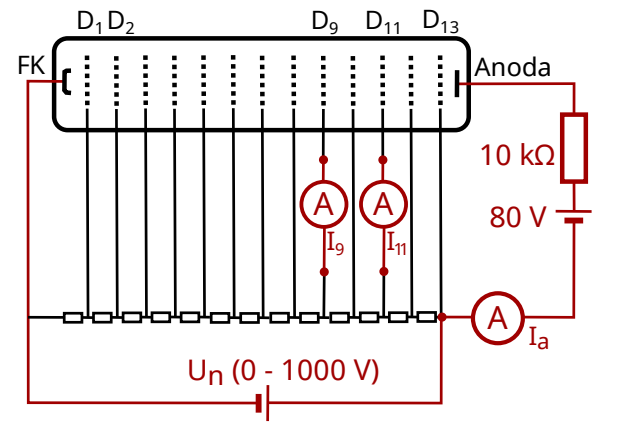
\includegraphics[width=0.5\textwidth]{fotonasobic.png}
    \caption{Schéma zapojení fotonásobiče. FK je fotokatoda, $ D_1 $ až $ D_{13} $ jsou dynody a $ U_n $ je napětí přivedené na násobič. }
\end{figure}

\newpage

\section{Výsledky měření}

\subsection{Závislost koeficientu sekundární emise na energii elektronů}

Fotonásobič jsem zapojil podle obrázku 1 a pro různé napětí $ U_n $ měřil anodový proud a proud na dynodě 10 a 12. Koeficient sekundární emise a energii dopadajících elektronů potom spočítám podle vztahů

\begin{equation}
\sigma = \sqrt{\frac{I_{12}}{I_{10}}} \quad \quad  \quad E = \frac{q U_n}{n},
\end{equation}

\noindent
protože mezi 10 a 12 dynodou dojede k zesílení o $ \sigma^{2} $ a napětí $ U_n $  je mezi dynody rozdělené rovnoměrně. Závislost $ \sigma $ na $ E $ by měla exponenciální podle vztahu (3), který tedy zlogaritmuju a fit bude přímkou podle $ y = \ln (\frac{\sigma}{E}) = f(E) $ pro směrnici $ \mu $ 

\begin{table}[htpb]
    \begin{minipage}[b]{.35\linewidth}
        \centering
        \begin{equation}
            \ln \frac{\sigma}{E} = -\mu E + \ln A
        \end{equation}
        \begin{align*}
            \mu_1 &= 0.0023 \pm 0.0004 \\
            \mu_3 &= 0.0022  \pm 0.0005  \\
            \mu_5 &= 0.0025 \pm 0.0004 \\
        \end{align*}
        \vspace{-30pt}
        \begin{align*}
            A_1 &= -2.56 \pm 0.02 \\
            A_3 &= -2.57 \pm 0.02 \\
            A_5 &= -2.56 \pm 0.02 \\
            \\
        \end{align*}
    \end{minipage} 
    \hfill
    \begin{minipage}[b]{.60\linewidth}
        \centering
        % GNUPLOT: LaTeX picture with Postscript
\begingroup
  \makeatletter
  \providecommand\color[2][]{%
    \GenericError{(gnuplot) \space\space\space\@spaces}{%
      Package color not loaded in conjunction with
      terminal option `colourtext'%
    }{See the gnuplot documentation for explanation.%
    }{Either use 'blacktext' in gnuplot or load the package
      color.sty in LaTeX.}%
    \renewcommand\color[2][]{}%
  }%
  \providecommand\includegraphics[2][]{%
    \GenericError{(gnuplot) \space\space\space\@spaces}{%
      Package graphicx or graphics not loaded%
    }{See the gnuplot documentation for explanation.%
    }{The gnuplot epslatex terminal needs graphicx.sty or graphics.sty.}%
    \renewcommand\includegraphics[2][]{}%
  }%
  \providecommand\rotatebox[2]{#2}%
  \@ifundefined{ifGPcolor}{%
    \newif\ifGPcolor
    \GPcolorfalse
  }{}%
  \@ifundefined{ifGPblacktext}{%
    \newif\ifGPblacktext
    \GPblacktexttrue
  }{}%
  % define a \g@addto@macro without @ in the name:
  \let\gplgaddtomacro\g@addto@macro
  % define empty templates for all commands taking text:
  \gdef\gplbacktext{}%
  \gdef\gplfronttext{}%
  \makeatother
  \ifGPblacktext
    % no textcolor at all
    \def\colorrgb#1{}%
    \def\colorgray#1{}%
  \else
    % gray or color?
    \ifGPcolor
      \def\colorrgb#1{\color[rgb]{#1}}%
      \def\colorgray#1{\color[gray]{#1}}%
      \expandafter\def\csname LTw\endcsname{\color{white}}%
      \expandafter\def\csname LTb\endcsname{\color{black}}%
      \expandafter\def\csname LTa\endcsname{\color{black}}%
      \expandafter\def\csname LT0\endcsname{\color[rgb]{1,0,0}}%
      \expandafter\def\csname LT1\endcsname{\color[rgb]{0,1,0}}%
      \expandafter\def\csname LT2\endcsname{\color[rgb]{0,0,1}}%
      \expandafter\def\csname LT3\endcsname{\color[rgb]{1,0,1}}%
      \expandafter\def\csname LT4\endcsname{\color[rgb]{0,1,1}}%
      \expandafter\def\csname LT5\endcsname{\color[rgb]{1,1,0}}%
      \expandafter\def\csname LT6\endcsname{\color[rgb]{0,0,0}}%
      \expandafter\def\csname LT7\endcsname{\color[rgb]{1,0.3,0}}%
      \expandafter\def\csname LT8\endcsname{\color[rgb]{0.5,0.5,0.5}}%
    \else
      % gray
      \def\colorrgb#1{\color{black}}%
      \def\colorgray#1{\color[gray]{#1}}%
      \expandafter\def\csname LTw\endcsname{\color{white}}%
      \expandafter\def\csname LTb\endcsname{\color{black}}%
      \expandafter\def\csname LTa\endcsname{\color{black}}%
      \expandafter\def\csname LT0\endcsname{\color{black}}%
      \expandafter\def\csname LT1\endcsname{\color{black}}%
      \expandafter\def\csname LT2\endcsname{\color{black}}%
      \expandafter\def\csname LT3\endcsname{\color{black}}%
      \expandafter\def\csname LT4\endcsname{\color{black}}%
      \expandafter\def\csname LT5\endcsname{\color{black}}%
      \expandafter\def\csname LT6\endcsname{\color{black}}%
      \expandafter\def\csname LT7\endcsname{\color{black}}%
      \expandafter\def\csname LT8\endcsname{\color{black}}%
    \fi
  \fi
    \setlength{\unitlength}{0.0500bp}%
    \ifx\gptboxheight\undefined%
      \newlength{\gptboxheight}%
      \newlength{\gptboxwidth}%
      \newsavebox{\gptboxtext}%
    \fi%
    \setlength{\fboxrule}{0.5pt}%
    \setlength{\fboxsep}{1pt}%
    \definecolor{tbcol}{rgb}{1,1,1}%
\begin{picture}(5328.00,3600.00)%
    \gplgaddtomacro\gplbacktext{%
      \csname LTb\endcsname%%
      \put(1078,704){\makebox(0,0)[r]{\strut{}$-2.71$}}%
      \put(1078,1038){\makebox(0,0)[r]{\strut{}$-2.7$}}%
      \put(1078,1373){\makebox(0,0)[r]{\strut{}$-2.69$}}%
      \put(1078,1707){\makebox(0,0)[r]{\strut{}$-2.68$}}%
      \put(1078,2041){\makebox(0,0)[r]{\strut{}$-2.67$}}%
      \put(1078,2376){\makebox(0,0)[r]{\strut{}$-2.66$}}%
      \put(1078,2710){\makebox(0,0)[r]{\strut{}$-2.65$}}%
      \put(1078,3045){\makebox(0,0)[r]{\strut{}$-2.64$}}%
      \put(1078,3379){\makebox(0,0)[r]{\strut{}$-2.63$}}%
      \put(1210,484){\makebox(0,0){\strut{}$42$}}%
      \put(1582,484){\makebox(0,0){\strut{}$44$}}%
      \put(1954,484){\makebox(0,0){\strut{}$46$}}%
      \put(2326,484){\makebox(0,0){\strut{}$48$}}%
      \put(2698,484){\makebox(0,0){\strut{}$50$}}%
      \put(3071,484){\makebox(0,0){\strut{}$52$}}%
      \put(3443,484){\makebox(0,0){\strut{}$54$}}%
      \put(3815,484){\makebox(0,0){\strut{}$56$}}%
      \put(4187,484){\makebox(0,0){\strut{}$58$}}%
      \put(4559,484){\makebox(0,0){\strut{}$60$}}%
      \put(4931,484){\makebox(0,0){\strut{}$62$}}%
    }%
    \gplgaddtomacro\gplfronttext{%
      \csname LTb\endcsname%%
      \put(209,2041){\rotatebox{-270}{\makebox(0,0){\strut{} $ I $ ($ \mu A$)}}}%
      \put(3070,154){\makebox(0,0){\strut{}$ U $ ($ V $)}}%
    }%
    \gplbacktext
    \put(0,0){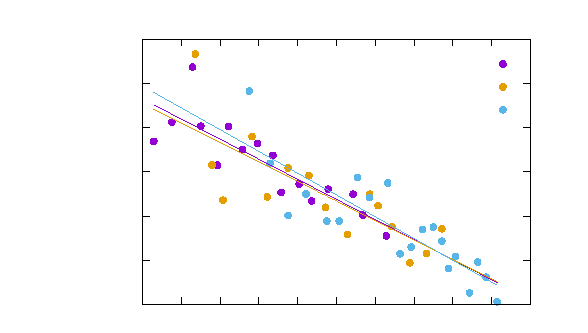
\includegraphics[width={266.40bp},height={180.00bp}]{sigma_na_U}}%
    \gplfronttext
  \end{picture}%
\endgroup

        \captionsetup{type=graph}
        \caption{Závislost koeficientu emise na energii dopadajících elektronů.}
    \end{minipage} 
\end{table}

\vspace{-10pt}

\begin{table}[htpb]
    \centering
    \footnotesize
    \makebox[\textwidth][c]{%
    
    \begin{tabular}{ | c c c c c c | c c c c c c | c c c c c c |}
        \hline
        \multicolumn{6}{|l}{poloha klínu 1 $ \Phi = 90 \ \mu  $Lm } & \multicolumn{6}{|l}{poloha klínu 3 $ \Phi = 52 \ \mu  $Lm} & \multicolumn{6}{|l|}{poloha klínu 5 $ \Phi = 33\ \mu  $Lm} \\ \hline
        $ U_n $ & $ I_{10} $ & $ I_{12} $ & $ I_a $ & $ \sigma $ & k $ \cdot 10^{-9} $  &
        $ U_n $ & $ I_{10} $ & $ I_{12} $ & $ I_a $ & $ \sigma $ & k $ \cdot 10^{-9} $&
        $ U_n $ & $ I_{10} $ & $ I_{12} $ & $ I_a $ & $ \sigma $ & k $ \cdot 10^{-9} $  \\ 
        V & $ \mu A $  & $ \mu A $ &  $ \mu A $ & & ALm$ ^{-1}$  &
        V & $ \mu A $  & $ \mu A $ &  $ \mu A $ & & $ALm ^{-1}$  &
        V & $ \mu A $  & $ \mu A $ &  $ \mu A $ & & ALm$ ^{-1}$  \\ 
        \hline
        596 & 0.16 & 1.38 & 10 & 2.94 & 31.0 & 626 & 0.12 & 1.18 & 9  & 3.15 & 20.4 & 665 & 0.15 & 1.69 & 12 & 3.32 & 18.1 \\
        609 & 0.18 & 1.64 & 12 & 3.02 & 25.8 & 638 & 0.13 & 1.33 & 11 & 3.13 & 24.5 & 680 & 0.16 & 1.84 & 14 & 3.34 & 19.4 \\
        624 & 0.20 & 1.96 & 14 & 3.13 & 18.0 & 645 & 0.17 & 1.63 & 12 & 3.14 & 25.1 & 693 & 0.18 & 1.99 & 16 & 3.36 & 20.1 \\
        630 & 0.21 & 2.04 & 15 & 3.12 & 20.4 & 666 & 0.20 & 2.15 & 18 & 3.29 & 19.7 & 705 & 0.20 & 2.40 & 18 & 3.44 & 16.3 \\
        642 & 0.24 & 2.38 & 18 & 3.15 & 21.2 & 677 & 0.25 & 2.69 & 19 & 3.30 & 20.0 & 720 & 0.21 & 2.57 & 22 & 3.49 & 16.2 \\
        650 & 0.26 & 2.69 & 20 & 3.22 & 17.5 & 693 & 0.25 & 2.86 & 21 & 3.40 & 15.5 & 730 & 0.26 & 3.23 & 24 & 3.54 & 14.8 \\
        660 & 0.29 & 3.06 & 24 & 3.25 & 18.3 & 708 & 0.29 & 3.47 & 27 & 3.46 & 14.5 & 743 & 0.27 & 3.61 & 28 & 3.63 & 11.7 \\
        671 & 0.31 & 3.39 & 26 & 3.31 & 15.4 & 719 & 0.31 & 3.84 & 31 & 3.50 & 14.5 & 751 & 0.32 & 4.23 & 32 & 3.66 & 12.1 \\
        682 & 0.34 & 3.82 & 30 & 3.35 & 14.7 & 736 & 0.39 & 4.95 & 38 & 3.55 & 14.3 & 765 & 0.32 & 4.51 & 36 & 3.74 & 10.2 \\
        688 & 0.37 & 4.16 & 33 & 3.35 & 16.1 & 751 & 0.49 & 6.60 & 46 & 3.66 & 11.3 & 773 & 0.38 & 5.31 & 40 & 3.72 & 12.1 \\
        701 & 0.43 & 5.04 & 40 & 3.42 & 14.6 & 758 & 0.47 & 6.43 & 49 & 3.68 & 11.3 & 782 & 0.37 & 5.31 & 44 & 3.77 & 11.2 \\
        710 & 0.45 & 5.37 & 44 & 3.45 & 14.2 & 768 & 0.52 & 7.23 & 54 & 3.71 & 11.1 & 790 & 0.39 & 5.62 & 48 & 3.82 & 10.1 \\
        722 & 0.52 & 6.45 & 53 & 3.52 & 13.0 & 780 & 0.61 & 8.56 & 66 & 3.75 & 11.8 & 797 & 0.43 & 6.43 & 52 & 3.86 & 9.41 \\
        740 & 0.60 & 7.80 & 66 & 3.61 & 11.7 & 793 & 0.66 & 9.60 & 79 & 3.81 & 11.1 & 804 & 0.48 & 7.28 & 57 & 3.88 & 9.70 \\
        747 & 0.65 & 8.53 & 74 & 3.62 & 12.2 & 804 & 0.65 & 9.89 & 90 & 3.89 & 9.73 & 808 & 0.50 & 7.49 & 60 & 3.88 & 10.2 \\
        764 & 0.75 & 10.2 & 90 & 3.69 & 11.6 &     &      &      &    &      &      & 814 & 0.54 & 8.22 & 64 & 3.91 & 9.61 \\
            &      &      &    &      &      &     &      &      &    &      &      & 824 & 0.62 & 9.53 & 72 & 3.93 & 10.2 \\
            &      &      &    &      &      &     &      &      &    &      &      & 829 & 0.64 & 10.1 & 79 & 3.98 & 9.20 \\
            &      &      &    &      &      &     &      &      &    &      &      & 835 & 0.75 & 12.0 & 84 & 4.00 & 9.28 \\
            &      &      &    &      &      &     &      &      &    &      &      & 843 & 0.70 & 11.3 & 90 & 4.01 & 9.41 \\
        \hline     
    \end{tabular}  
    }
    \caption{Změřené anodové a dynodové proudy při různých napětích na fotonásobiči.}
\end{table}        

Z tabulky 1 můžeme taky vypočítat podle vztahů (6) a (7) zesílení $ M $ a citlivosti $ S $ a vynést je v závislost na napětí $ U_n $. Obě tyto závislosti by měli být znovu podle vztahu (3) přibližně exponenciální 
                   
\begin{table}[htpb]
    \begin{minipage}[b]{.45\linewidth}
        \centering
        % GNUPLOT: LaTeX picture with Postscript
\begingroup
  \makeatletter
  \providecommand\color[2][]{%
    \GenericError{(gnuplot) \space\space\space\@spaces}{%
      Package color not loaded in conjunction with
      terminal option `colourtext'%
    }{See the gnuplot documentation for explanation.%
    }{Either use 'blacktext' in gnuplot or load the package
      color.sty in LaTeX.}%
    \renewcommand\color[2][]{}%
  }%
  \providecommand\includegraphics[2][]{%
    \GenericError{(gnuplot) \space\space\space\@spaces}{%
      Package graphicx or graphics not loaded%
    }{See the gnuplot documentation for explanation.%
    }{The gnuplot epslatex terminal needs graphicx.sty or graphics.sty.}%
    \renewcommand\includegraphics[2][]{}%
  }%
  \providecommand\rotatebox[2]{#2}%
  \@ifundefined{ifGPcolor}{%
    \newif\ifGPcolor
    \GPcolorfalse
  }{}%
  \@ifundefined{ifGPblacktext}{%
    \newif\ifGPblacktext
    \GPblacktexttrue
  }{}%
  % define a \g@addto@macro without @ in the name:
  \let\gplgaddtomacro\g@addto@macro
  % define empty templates for all commands taking text:
  \gdef\gplbacktext{}%
  \gdef\gplfronttext{}%
  \makeatother
  \ifGPblacktext
    % no textcolor at all
    \def\colorrgb#1{}%
    \def\colorgray#1{}%
  \else
    % gray or color?
    \ifGPcolor
      \def\colorrgb#1{\color[rgb]{#1}}%
      \def\colorgray#1{\color[gray]{#1}}%
      \expandafter\def\csname LTw\endcsname{\color{white}}%
      \expandafter\def\csname LTb\endcsname{\color{black}}%
      \expandafter\def\csname LTa\endcsname{\color{black}}%
      \expandafter\def\csname LT0\endcsname{\color[rgb]{1,0,0}}%
      \expandafter\def\csname LT1\endcsname{\color[rgb]{0,1,0}}%
      \expandafter\def\csname LT2\endcsname{\color[rgb]{0,0,1}}%
      \expandafter\def\csname LT3\endcsname{\color[rgb]{1,0,1}}%
      \expandafter\def\csname LT4\endcsname{\color[rgb]{0,1,1}}%
      \expandafter\def\csname LT5\endcsname{\color[rgb]{1,1,0}}%
      \expandafter\def\csname LT6\endcsname{\color[rgb]{0,0,0}}%
      \expandafter\def\csname LT7\endcsname{\color[rgb]{1,0.3,0}}%
      \expandafter\def\csname LT8\endcsname{\color[rgb]{0.5,0.5,0.5}}%
    \else
      % gray
      \def\colorrgb#1{\color{black}}%
      \def\colorgray#1{\color[gray]{#1}}%
      \expandafter\def\csname LTw\endcsname{\color{white}}%
      \expandafter\def\csname LTb\endcsname{\color{black}}%
      \expandafter\def\csname LTa\endcsname{\color{black}}%
      \expandafter\def\csname LT0\endcsname{\color{black}}%
      \expandafter\def\csname LT1\endcsname{\color{black}}%
      \expandafter\def\csname LT2\endcsname{\color{black}}%
      \expandafter\def\csname LT3\endcsname{\color{black}}%
      \expandafter\def\csname LT4\endcsname{\color{black}}%
      \expandafter\def\csname LT5\endcsname{\color{black}}%
      \expandafter\def\csname LT6\endcsname{\color{black}}%
      \expandafter\def\csname LT7\endcsname{\color{black}}%
      \expandafter\def\csname LT8\endcsname{\color{black}}%
    \fi
  \fi
    \setlength{\unitlength}{0.0500bp}%
    \ifx\gptboxheight\undefined%
      \newlength{\gptboxheight}%
      \newlength{\gptboxwidth}%
      \newsavebox{\gptboxtext}%
    \fi%
    \setlength{\fboxrule}{0.5pt}%
    \setlength{\fboxsep}{1pt}%
    \definecolor{tbcol}{rgb}{1,1,1}%
\begin{picture}(5040.00,2880.00)%
    \gplgaddtomacro\gplbacktext{%
      \csname LTb\endcsname%%
      \put(814,201){\makebox(0,0)[r]{\strut{}$0$}}%
      \put(814,611){\makebox(0,0)[r]{\strut{}$50$}}%
      \put(814,1020){\makebox(0,0)[r]{\strut{}$100$}}%
      \put(814,1430){\makebox(0,0)[r]{\strut{}$150$}}%
      \put(814,1840){\makebox(0,0)[r]{\strut{}$200$}}%
      \put(814,2249){\makebox(0,0)[r]{\strut{}$250$}}%
      \put(814,2659){\makebox(0,0)[r]{\strut{}$300$}}%
      \put(946,-19){\makebox(0,0){\strut{}$550$}}%
      \put(1562,-19){\makebox(0,0){\strut{}$600$}}%
      \put(2178,-19){\makebox(0,0){\strut{}$650$}}%
      \put(2795,-19){\makebox(0,0){\strut{}$700$}}%
      \put(3411,-19){\makebox(0,0){\strut{}$750$}}%
      \put(4027,-19){\makebox(0,0){\strut{}$800$}}%
      \put(4643,-19){\makebox(0,0){\strut{}$850$}}%
    }%
    \gplgaddtomacro\gplfronttext{%
      \csname LTb\endcsname%%
      \put(209,1430){\rotatebox{-270}{\makebox(0,0){\strut{}M $ \cdot 10^6 $ }}}%
      \put(2794,-349){\makebox(0,0){\strut{}$U_n$ (V)}}%
      \csname LTb\endcsname%%
      \put(2134,2486){\makebox(0,0)[r]{\strut{}poloha 1}}%
      \csname LTb\endcsname%%
      \put(2134,2266){\makebox(0,0)[r]{\strut{}poloha 3}}%
      \csname LTb\endcsname%%
      \put(2134,2046){\makebox(0,0)[r]{\strut{}poloha 5}}%
    }%
    \gplbacktext
    \put(0,0){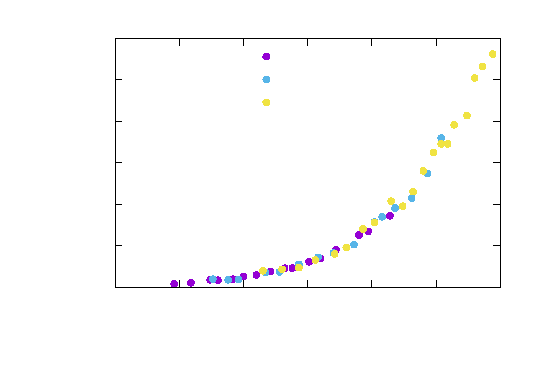
\includegraphics[width={252.00bp},height={144.00bp}]{M}}%
    \gplfronttext
  \end{picture}%
\endgroup

        \captionsetup{type=graph}
        \caption{Závislost zesílení fotonásobiče na napětí $ U_n $}
    \end{minipage} 
    \hfill
    \begin{minipage}[b]{.45\linewidth}
        \centering
        % GNUPLOT: LaTeX picture with Postscript
\begingroup
  \makeatletter
  \providecommand\color[2][]{%
    \GenericError{(gnuplot) \space\space\space\@spaces}{%
      Package color not loaded in conjunction with
      terminal option `colourtext'%
    }{See the gnuplot documentation for explanation.%
    }{Either use 'blacktext' in gnuplot or load the package
      color.sty in LaTeX.}%
    \renewcommand\color[2][]{}%
  }%
  \providecommand\includegraphics[2][]{%
    \GenericError{(gnuplot) \space\space\space\@spaces}{%
      Package graphicx or graphics not loaded%
    }{See the gnuplot documentation for explanation.%
    }{The gnuplot epslatex terminal needs graphicx.sty or graphics.sty.}%
    \renewcommand\includegraphics[2][]{}%
  }%
  \providecommand\rotatebox[2]{#2}%
  \@ifundefined{ifGPcolor}{%
    \newif\ifGPcolor
    \GPcolorfalse
  }{}%
  \@ifundefined{ifGPblacktext}{%
    \newif\ifGPblacktext
    \GPblacktexttrue
  }{}%
  % define a \g@addto@macro without @ in the name:
  \let\gplgaddtomacro\g@addto@macro
  % define empty templates for all commands taking text:
  \gdef\gplbacktext{}%
  \gdef\gplfronttext{}%
  \makeatother
  \ifGPblacktext
    % no textcolor at all
    \def\colorrgb#1{}%
    \def\colorgray#1{}%
  \else
    % gray or color?
    \ifGPcolor
      \def\colorrgb#1{\color[rgb]{#1}}%
      \def\colorgray#1{\color[gray]{#1}}%
      \expandafter\def\csname LTw\endcsname{\color{white}}%
      \expandafter\def\csname LTb\endcsname{\color{black}}%
      \expandafter\def\csname LTa\endcsname{\color{black}}%
      \expandafter\def\csname LT0\endcsname{\color[rgb]{1,0,0}}%
      \expandafter\def\csname LT1\endcsname{\color[rgb]{0,1,0}}%
      \expandafter\def\csname LT2\endcsname{\color[rgb]{0,0,1}}%
      \expandafter\def\csname LT3\endcsname{\color[rgb]{1,0,1}}%
      \expandafter\def\csname LT4\endcsname{\color[rgb]{0,1,1}}%
      \expandafter\def\csname LT5\endcsname{\color[rgb]{1,1,0}}%
      \expandafter\def\csname LT6\endcsname{\color[rgb]{0,0,0}}%
      \expandafter\def\csname LT7\endcsname{\color[rgb]{1,0.3,0}}%
      \expandafter\def\csname LT8\endcsname{\color[rgb]{0.5,0.5,0.5}}%
    \else
      % gray
      \def\colorrgb#1{\color{black}}%
      \def\colorgray#1{\color[gray]{#1}}%
      \expandafter\def\csname LTw\endcsname{\color{white}}%
      \expandafter\def\csname LTb\endcsname{\color{black}}%
      \expandafter\def\csname LTa\endcsname{\color{black}}%
      \expandafter\def\csname LT0\endcsname{\color{black}}%
      \expandafter\def\csname LT1\endcsname{\color{black}}%
      \expandafter\def\csname LT2\endcsname{\color{black}}%
      \expandafter\def\csname LT3\endcsname{\color{black}}%
      \expandafter\def\csname LT4\endcsname{\color{black}}%
      \expandafter\def\csname LT5\endcsname{\color{black}}%
      \expandafter\def\csname LT6\endcsname{\color{black}}%
      \expandafter\def\csname LT7\endcsname{\color{black}}%
      \expandafter\def\csname LT8\endcsname{\color{black}}%
    \fi
  \fi
    \setlength{\unitlength}{0.0500bp}%
    \ifx\gptboxheight\undefined%
      \newlength{\gptboxheight}%
      \newlength{\gptboxwidth}%
      \newsavebox{\gptboxtext}%
    \fi%
    \setlength{\fboxrule}{0.5pt}%
    \setlength{\fboxsep}{1pt}%
    \definecolor{tbcol}{rgb}{1,1,1}%
\begin{picture}(5040.00,3310.00)%
    \gplgaddtomacro\gplbacktext{%
      \csname LTb\endcsname%%
      \put(946,704){\makebox(0,0)[r]{\strut{}$-2.5$}}%
      \put(946,1045){\makebox(0,0)[r]{\strut{}$-2$}}%
      \put(946,1385){\makebox(0,0)[r]{\strut{}$-1.5$}}%
      \put(946,1726){\makebox(0,0)[r]{\strut{}$-1$}}%
      \put(946,2067){\makebox(0,0)[r]{\strut{}$-0.5$}}%
      \put(946,2408){\makebox(0,0)[r]{\strut{}$0$}}%
      \put(946,2748){\makebox(0,0)[r]{\strut{}$0.5$}}%
      \put(946,3089){\makebox(0,0)[r]{\strut{}$1$}}%
      \put(1078,484){\makebox(0,0){\strut{}$550$}}%
      \put(1672,484){\makebox(0,0){\strut{}$600$}}%
      \put(2266,484){\makebox(0,0){\strut{}$650$}}%
      \put(2861,484){\makebox(0,0){\strut{}$700$}}%
      \put(3455,484){\makebox(0,0){\strut{}$750$}}%
      \put(4049,484){\makebox(0,0){\strut{}$800$}}%
      \put(4643,484){\makebox(0,0){\strut{}$850$}}%
    }%
    \gplgaddtomacro\gplfronttext{%
      \csname LTb\endcsname%%
      \put(209,1896){\rotatebox{-270}{\makebox(0,0){\strut{} log($ S $) (A Lm$^{-1} $) }}}%
      \put(2860,154){\makebox(0,0){\strut{}$U_n$ (V)}}%
      \csname LTb\endcsname%%
      \put(2266,2916){\makebox(0,0)[r]{\strut{}poloha 1}}%
      \csname LTb\endcsname%%
      \put(2266,2696){\makebox(0,0)[r]{\strut{}poloha 3}}%
      \csname LTb\endcsname%%
      \put(2266,2476){\makebox(0,0)[r]{\strut{}poloha 5}}%
    }%
    \gplbacktext
    \put(0,0){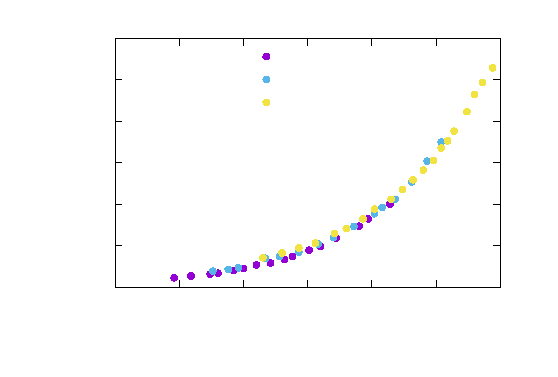
\includegraphics[width={252.00bp},height={165.50bp}]{S}}%
    \gplfronttext
  \end{picture}%
\endgroup

        \captionsetup{type=graph}
        \caption{Závislost citlivosti fotonásobiče na napětí $ U_n $ }
    \end{minipage} 
\end{table}
\subsection{Závislost koeficientu sekundární emise na osvětlení fotokatody}
                   
Tentokrát jsem nechal stálé napětí $ U_n = $ a pohyboval s klínem pro regulaci osvětlení fotokatody. Naměřená data jsou uvedené v tabulce 2 a 3 a závislost koeficientu sekundární emise $ \sigma $  na osvětlení $ \Phi $ vykreslená do grafu 4. Koeficient emise katody na osvětlení tolik nezávisí, takže jsem hodnoty statisticky vyhodnotil a vypočítal společně s integrální citlivostí fotokatody $ k $ ze vztahů (4) a (5).

\begin{align*}
    \sigma &= 3.68 \pm 0.05 && k = 11 \pm 2 \text{ nALm}  ^{-1} && \text{pro $ U_n = 750 $ V} \\
    \sigma &= 3.26 \pm 0.08 && k = 18 \pm 5 \text{ nALm}^{-1} && \text{pro $ U_n = 650 $ V }
\end{align*}

\begin{figure}[htpb]
    \centering
    % GNUPLOT: LaTeX picture with Postscript
\begingroup
  \makeatletter
  \providecommand\color[2][]{%
    \GenericError{(gnuplot) \space\space\space\@spaces}{%
      Package color not loaded in conjunction with
      terminal option `colourtext'%
    }{See the gnuplot documentation for explanation.%
    }{Either use 'blacktext' in gnuplot or load the package
      color.sty in LaTeX.}%
    \renewcommand\color[2][]{}%
  }%
  \providecommand\includegraphics[2][]{%
    \GenericError{(gnuplot) \space\space\space\@spaces}{%
      Package graphicx or graphics not loaded%
    }{See the gnuplot documentation for explanation.%
    }{The gnuplot epslatex terminal needs graphicx.sty or graphics.sty.}%
    \renewcommand\includegraphics[2][]{}%
  }%
  \providecommand\rotatebox[2]{#2}%
  \@ifundefined{ifGPcolor}{%
    \newif\ifGPcolor
    \GPcolorfalse
  }{}%
  \@ifundefined{ifGPblacktext}{%
    \newif\ifGPblacktext
    \GPblacktexttrue
  }{}%
  % define a \g@addto@macro without @ in the name:
  \let\gplgaddtomacro\g@addto@macro
  % define empty templates for all commands taking text:
  \gdef\gplbacktext{}%
  \gdef\gplfronttext{}%
  \makeatother
  \ifGPblacktext
    % no textcolor at all
    \def\colorrgb#1{}%
    \def\colorgray#1{}%
  \else
    % gray or color?
    \ifGPcolor
      \def\colorrgb#1{\color[rgb]{#1}}%
      \def\colorgray#1{\color[gray]{#1}}%
      \expandafter\def\csname LTw\endcsname{\color{white}}%
      \expandafter\def\csname LTb\endcsname{\color{black}}%
      \expandafter\def\csname LTa\endcsname{\color{black}}%
      \expandafter\def\csname LT0\endcsname{\color[rgb]{1,0,0}}%
      \expandafter\def\csname LT1\endcsname{\color[rgb]{0,1,0}}%
      \expandafter\def\csname LT2\endcsname{\color[rgb]{0,0,1}}%
      \expandafter\def\csname LT3\endcsname{\color[rgb]{1,0,1}}%
      \expandafter\def\csname LT4\endcsname{\color[rgb]{0,1,1}}%
      \expandafter\def\csname LT5\endcsname{\color[rgb]{1,1,0}}%
      \expandafter\def\csname LT6\endcsname{\color[rgb]{0,0,0}}%
      \expandafter\def\csname LT7\endcsname{\color[rgb]{1,0.3,0}}%
      \expandafter\def\csname LT8\endcsname{\color[rgb]{0.5,0.5,0.5}}%
    \else
      % gray
      \def\colorrgb#1{\color{black}}%
      \def\colorgray#1{\color[gray]{#1}}%
      \expandafter\def\csname LTw\endcsname{\color{white}}%
      \expandafter\def\csname LTb\endcsname{\color{black}}%
      \expandafter\def\csname LTa\endcsname{\color{black}}%
      \expandafter\def\csname LT0\endcsname{\color{black}}%
      \expandafter\def\csname LT1\endcsname{\color{black}}%
      \expandafter\def\csname LT2\endcsname{\color{black}}%
      \expandafter\def\csname LT3\endcsname{\color{black}}%
      \expandafter\def\csname LT4\endcsname{\color{black}}%
      \expandafter\def\csname LT5\endcsname{\color{black}}%
      \expandafter\def\csname LT6\endcsname{\color{black}}%
      \expandafter\def\csname LT7\endcsname{\color{black}}%
      \expandafter\def\csname LT8\endcsname{\color{black}}%
    \fi
  \fi
    \setlength{\unitlength}{0.0500bp}%
    \ifx\gptboxheight\undefined%
      \newlength{\gptboxheight}%
      \newlength{\gptboxwidth}%
      \newsavebox{\gptboxtext}%
    \fi%
    \setlength{\fboxrule}{0.5pt}%
    \setlength{\fboxsep}{1pt}%
    \definecolor{tbcol}{rgb}{1,1,1}%
\begin{picture}(5040.00,3310.00)%
    \gplgaddtomacro\gplbacktext{%
      \csname LTb\endcsname%%
      \put(814,704){\makebox(0,0)[r]{\strut{}$3.1$}}%
      \put(814,1045){\makebox(0,0)[r]{\strut{}$3.2$}}%
      \put(814,1385){\makebox(0,0)[r]{\strut{}$3.3$}}%
      \put(814,1726){\makebox(0,0)[r]{\strut{}$3.4$}}%
      \put(814,2067){\makebox(0,0)[r]{\strut{}$3.5$}}%
      \put(814,2408){\makebox(0,0)[r]{\strut{}$3.6$}}%
      \put(814,2748){\makebox(0,0)[r]{\strut{}$3.7$}}%
      \put(814,3089){\makebox(0,0)[r]{\strut{}$3.8$}}%
      \put(946,484){\makebox(0,0){\strut{}$10$}}%
      \put(1357,484){\makebox(0,0){\strut{}$20$}}%
      \put(1768,484){\makebox(0,0){\strut{}$30$}}%
      \put(2178,484){\makebox(0,0){\strut{}$40$}}%
      \put(2589,484){\makebox(0,0){\strut{}$50$}}%
      \put(3000,484){\makebox(0,0){\strut{}$60$}}%
      \put(3411,484){\makebox(0,0){\strut{}$70$}}%
      \put(3821,484){\makebox(0,0){\strut{}$80$}}%
      \put(4232,484){\makebox(0,0){\strut{}$90$}}%
      \put(4643,484){\makebox(0,0){\strut{}$100$}}%
    }%
    \gplgaddtomacro\gplfronttext{%
      \csname LTb\endcsname%%
      \put(209,1896){\rotatebox{-270}{\makebox(0,0){\strut{}$ \sigma $}}}%
      \put(2794,154){\makebox(0,0){\strut{}$ \Phi $ ($\mu$Lm)}}%
      \csname LTb\endcsname%%
      \put(3933,2025){\makebox(0,0)[r]{\strut{}$U_n = 650$V}}%
      \csname LTb\endcsname%%
      \put(3933,1805){\makebox(0,0)[r]{\strut{}$U_n = 750$V}}%
    }%
    \gplbacktext
    \put(0,0){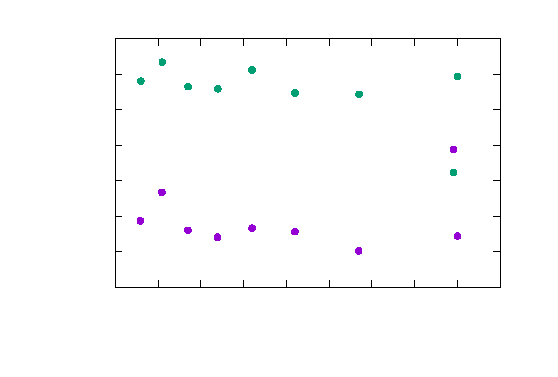
\includegraphics[width={252.00bp},height={165.50bp}]{sigma_na_phi}}%
    \gplfronttext
  \end{picture}%
\endgroup

    \captionsetup{type=graph}
    \caption{Závislost koeficientu sekundární emise na intenzitě osvětlení fotokatody}
\end{figure} 

\begin{table}[htpb]
    \centering
    \begin{tabular}{| c c | c c c c c |}
        \hline
        \multicolumn{2}{|l|}{} & \multicolumn{5}{l|}{$ U_n = 750 $ V} \\\hline
        klín & $ \Phi $ ($ \mu $Lm) & $ I_{10} $ $ (\mu A) $  & $ I_{12} $ $ (\mu A) $ & $ I_a $ $ (\mu A) $ & $ \sigma $ & $ k \cdot 10^{-9} $ (ALm$^{-1}  $ )  \\ \hline
        1 & 90 & 0.65 & 8.86 & 74 & 3.69 &  9.4 \\
        2 & 66 & 0.48 & 6.37 & 56 & 3.64 & 11.5 \\
        3 & 52 & 0.40 & 5.32 & 46 & 3.65 & 12.0 \\
        4 & 42 & 0.33 & 4.55 & 37 & 3.71 &  9.4 \\
        5 & 33 & 0.27 & 3.61 & 32 & 3.66 & 12.2 \\
        6 & 27 & 0.22 & 2.95 & 25 & 3.66 & 11.8 \\
        7 & 20 & 0.17 & 2.37 & 21 & 3.73 &  9.8 \\
        8 & 15 & 0.14 & 1.90 & 17 & 3.68 & 12.7 \\
        \hline
    \end{tabular}
    \caption{Změřené anodové a dynodové proudy při napětí $ U_n = 750 $ V .}
\end{table}

\begin{table}[htpb]
    \centering
    \begin{tabular}{| c c | c c c c c |}
        \hline
        \multicolumn{2}{|l|}{} & \multicolumn{5}{l|}{$ U_n = 650 $ V} \\\hline
        klín & $ \Phi $ ($ \mu $Lm) & $ I_{10} $ $ (\mu A) $  & $ I_{12} $ $ (\mu A) $ & $ I_a $ $ (\mu A) $ & $ \sigma $ & $ k \cdot 10^{-9} $ (ALm$^{-1}  $ ) \\ \hline
        1 & 90 & 0.24 & 2.57 & 20 & 3.24 & 15.6 \\
        2 & 66 & 0.21 & 2.12 & 16 & 3.20 & 20.1 \\
        3 & 52 & 0.16 & 1.70 & 13 & 3.26 & 16.6 \\
        4 & 42 & 0.11 & 1.18 & 11 & 3.27 & 16.7 \\
        5 & 33 & 0.12 & 1.27 & 10 & 3.24 & 21.0 \\
        6 & 27 & 0.11 & 1.15 & 9  & 3.26 & 21.8 \\
        7 & 20 & 0.07 & 0.85 & 7  & 3.37 & 13.9 \\
        8 & 15 & 0.07 & 0.78 & 6  & 3.29 & 22.0 \\
        \hline
    \end{tabular}
    \caption{Změřené anodové a dynodové proudy při napětí $ U_n = 650 $ V .}
\end{table}

\subsection{Vliv temného proudu}

Nakonec ještě ověřím vliv temného proudu na změřené hodnoty. Pro několik vysokých napětí jsem při vypnutém zdroji světla měřil anodový proud a hodnoty uvedl v tabulce 4. Všechny tyto proudy jsou mnohem nižší, než ty z předešlích tabulek, takže jej nebylo potřeba brát v úvahu.

\begin{table}[htpb]
    \centering
    \begin{tabular}{c l}
        $ U_n $  & $ I_a $  \\\hline
        1000 & 1 \\
        800  & 0.9 \\
        700  & 0.25 \\
    \end{tabular} 
    \caption{Anodový proud při nulovém osvětlení}
\end{table}


\section{Závěr}

V první části úlohy jsem měřil koeficient sekundární emise $ \sigma $ mezi dvěma dynodami fotonásobiče a ověřil, že na energii elektronů závisí exponenciálně podle vztahu $ \sigma = A E \exp (-\mu E) $. 
Z naměřených hodnot jsem potom taky dopočítal zesílení $ M $ a citlivost fotonásobiče $ S $ a hodnoty vynesl do grafů 2, a 3 v závislosti na napětí $ U_n $ .

Pomocí anodového proudu a zjištěného koeficientu sekundární emise jsem potom dopočítal fotokatodový proud $ I_f = I_a \sigma^{-n} $ a pak za vztahu (5) vyjádřil citlivost fotokatody $ k $ . Podle Stoletova zákona by mělo $ k $ záviset pouze na vlnové délce dopadajícího světla, ale z tabulek 2 a 3 vyplývá, že s rostoucím napětím na násobiči citlivost klesá. Myslím, že hodnoty $ I_f $ v těchto výpočtech nemůžou být příliš spolehlivé, když ani tímto způsobem většinou v tabulkách nedostanu sloupce $ I_{12} $ z $ I_{12} = I_a \sigma^{-2} $.










\begin{thebibliography}{0}
\bibitem{tabulky} Návod k úloze ~\url{https://is.muni.cz/auth/el/sci/jaro2025/F4210/um/fp3-9_fotonasobic.pdf}.   
\end{thebibliography}

\end{document}
